\chapter{Tag 18 — Kodierungs-Modi: Digit-Paar und C40}

\begin{quote}
Greta hat ihren Datamatrix-Encoder zur Reife gebracht. Heute, am letzten
Praktikumstag, schaut sie auf eine konkrete Frage: Darf es auch etwas
kleiner sein? Ein Symbol für die Seriennummer \texttt{12345678} wirkt
aufgebläht — jede Ziffer nimmt ein ganzes Codeword, obwohl man doch weiß,
dass hinter \texttt{1} und \texttt{2} immer genau zehn Möglichkeiten folgen.
\end{quote}

\section*{Lernziele für heute}

Am Ende von Tag 18 kannst du \dots

\begin{itemize}
\item erklären, warum ASCII-Modus bei Ziffernfolgen verschwenderisch ist
\item den Digit-Paar-Modus anwenden: zwei Ziffern als ein Codeword
  (Wert~$130 + d_1 \cdot 10 + d_2$)
\item den C40-Modus nachvollziehen: drei Zeichen aus $\{$A–Z, 0–9, Leerzeichen$\}$
  in zwei Codewords, mit Latch~(230) und Unlatch~(254)
\item die Funktion \texttt{kodiere\_smart()} schreiben, die automatisch den
  platzsparenden Modus wählt
\item die fertige \texttt{DatamatrixEncoderModi}-Klasse einsetzen
\end{itemize}

\paragraph{Material} Laptop mit Thonny und allen Bibliotheken aus den Vortagen.

% =============================================================
\section{Das Kapazitätsproblem bei Ziffernfolgen \normalfont(\textit{≈ 10 min})}
% =============================================================

Greta öffnet ihren Encoder und tippt:

\begin{minted}{python}
from encoder_klasse import DatamatrixEncoder
e = DatamatrixEncoder("12345678")
print(e)
# → DatamatrixEncoder(text='12345678', 14×14, 8+10 Codewords)
\end{minted}

Acht Ziffern brauchen acht Codewords und landen in einem \textbf{14×14}-Symbol.
Dabei steckt jede Ziffer $d$ als $\text{ord}(d)+1$ im Codeword — die Werte
\texttt{"0"} bis \texttt{"9"} liegen bei 49 bis 58.

Aber: Wenn zwei Ziffern zusammenkommen, weiß man schon vor dem Lesen, dass
es sich nur um Kombinationen \texttt{00} bis \texttt{99} handelt — genau
$10 \times 10 = 100$ Möglichkeiten. Und 100 Möglichkeiten passen
bequem in ein einziges Byte (das 256 Möglichkeiten hat). Der
Datamatrix-Standard nutzt das aus: Er definiert den
\textbf{Digit-Paar-Modus}.

% =============================================================
\section{Digit-Paar-Modus \normalfont(\textit{≈ 20 min})}
% =============================================================

Die Idee ist einfach:

\begin{center}
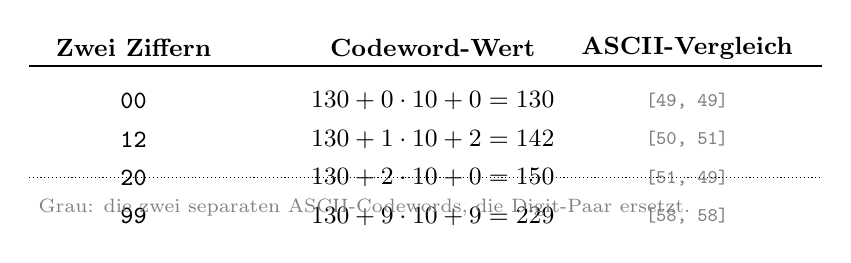
\begin{tikzpicture}[x=1.9cm, y=0.75cm, font=\small]
  % Kopfzeile
  \node[font=\small\bfseries] at (0.5, 2.2) {Zwei Ziffern};
  \node[font=\small\bfseries] at (2.5, 2.2) {Codeword-Wert};
  \node[font=\small\bfseries] at (4.2, 2.2) {ASCII-Vergleich};
  \draw[thick] (-0.2, 1.9) -- (5.1, 1.9);

  % Tabellenzeilen
  \foreach \za/\zb/\cw/\asc [count=\r from 0] in {
    0/0/130/{49, 49},
    1/2/142/{50, 51},
    2/0/150/{51, 49},
    9/9/229/{58, 58}%
  } {
    \pgfmathsetmacro{\y}{1.3 - \r * 0.65}
    \node at (0.5, \y) {\texttt{\za\zb}};
    \node at (2.5, \y) {$130 + \za \cdot 10 + \zb = \cw$};
    \node[font=\scriptsize, gray] at (4.2, \y) {\texttt{[\asc]}};
  }
  % Trennlinie vor letzter Zeile
  \draw[densely dotted] (-0.2, 0.0) -- (5.1, 0.0);
  % Legende
  \node[anchor=west, font=\scriptsize, gray] at (-0.2, -0.5)
    {Grau: die zwei separaten ASCII-Codewords, die Digit-Paar ersetzt.};
\end{tikzpicture}
\end{center}

Die Formel:
\[
  \text{CW} = 130 + d_1 \times 10 + d_2
  \qquad
  (d_1, d_2 \in \{0, \dots, 9\},\quad \text{CW} \in 130 \text{–} 229)
\]

Der Wertebereich~130–229 ist im Standard reserviert — er überlappt
nicht mit normalen ASCII-Codewords (1–128) und nicht mit den
Modus-Steuerbytes (230, 254~\dots).

\subsection*{Dekodierung — rückwärts}

Ein Scanner liest Codeword~142 und prüft: liegt es zwischen 130 und~229?
Ja. Also:
\[
  142 - 130 = 12 \quad\Rightarrow\quad d_1 = 12 \div 10 = 1,\quad
  d_2 = 12 \bmod 10 = 2 \quad\Rightarrow\quad \texttt{"12"}
\]

\begin{bleistiftuebung}
\textbf{Bleistift-Übung 1: Datum komprimieren}

Greta möchte das Datum \texttt{20251231} (8~Ziffern) im Digit-Paar-Modus kodieren.

\begin{enumerate}[label=\alph*)]
\item Kodiere \texttt{20251231} von Hand: schreibe für jedes Ziffernpaar
  das Codeword auf.
\item Wie viele Codewords entstehen? Vergleiche mit ASCII-Kodierung.
\item Das Symbol soll nur das Datum enthalten. Welche Symbolgröße
  wählt der Encoder? (Symboltabelle: 10×10 = 3~CW, 12×12 = 5~CW,
  14×14 = 8~CW)
\item Bonus: Was ergibt sich für \texttt{2025122} (sieben Ziffern —
  ungerade Anzahl)?
\end{enumerate}
\end{bleistiftuebung}

% =============================================================
\section{C40-Modus \normalfont(\textit{≈ 30 min})}
% =============================================================

Ziffern lassen sich mit Digit-Paar verdichten. Gibt es eine analoge
Abkürzung für Buchstaben?

Ja: den \textbf{C40-Modus}. Er kodiert drei Zeichen aus dem Satz
\{A–Z, 0–9, Leerzeichen\} in \textbf{zwei Codewords} — statt drei in
ASCII. Das entspricht einem Kompressionsfaktor von $3/2$. Im Gegenzug
braucht der Modus ein Steuerbyte vor und nach dem Segment.

\subsection*{C40-Werte}

Jedes Zeichen hat einen C40-Wert:

\begin{center}
\begin{tabular}{llll}
\hline
\textbf{Zeichen} & \textbf{C40-Wert} & \quad &
\textbf{Beispiele} \\
\hline
Leerzeichen      & 3                 & & \texttt{' '} → 3 \\
\texttt{'0'–'9'} & 4 bis 13          & & \texttt{'3'} → 7 \\
\texttt{'A'–'Z'} & 14 bis 39         & & \texttt{'A'} → 14, \texttt{'Z'} → 39 \\
\hline
\end{tabular}
\end{center}

\subsection*{Drei Zeichen → zwei Codewords}

Gegeben drei C40-Werte $V_1, V_2, V_3$:

\begin{align*}
  \mathit{tmp}    &= V_1 \times 1600 + V_2 \times 40 + V_3 + 1 \\
  \text{CW}_1 &= \mathit{tmp} \gg 8 \quad\text{(obere 8~Bit)} \\
  \text{CW}_2 &= \mathit{tmp} \mathbin{\&} \texttt{0xFF} \quad\text{(untere 8~Bit)}
\end{align*}

Beispiel für \textbf{GRE}:
$G=21,\; R=31,\; E=18$

\[
  \mathit{tmp} = 21 \times 1600 + 31 \times 40 + 18 + 1
              = 33600 + 1240 + 18 + 1 = 34859
\]
\[
  \text{CW}_1 = 34859 \div 256 = 136 \quad
  \text{CW}_2 = 34859 \bmod 256 = 43
\]

\subsection*{Latch und Unlatch}

Ein C40-Segment wird durch Steuerbytes eingerahmt:

\begin{center}
\texttt{[\,\textbf{230}\,|\; Daten-CWs \;|\,\textbf{254}\,]}
\end{center}

\begin{description}
\item[\texttt{230}] Latch: „Ab hier C40-Modus"
\item[\texttt{254}] Unlatch: „Zurück zu ASCII"
\end{description}

Restzeichen, die kein vollständiges Dreiertriplet bilden, werden nach
dem Unlatch wieder im ASCII-Modus angehängt.

\begin{bleistiftuebung}
\textbf{Bleistift-Übung 2: C40 lohnt sich — oder nicht?}

Kodiere \textbf{GRETA} (5~Buchstaben) im C40-Modus. G=21, R=31, E=18, T=33, A=14.

\begin{enumerate}[label=\alph*)]
\item Wie viele vollständige Dreiertriplets gibt es in \texttt{GRETA}?
  Welche Zeichen verbleiben als Rest?
\item Berechne die Codewords für das erste (und einzige) Triplet
  \texttt{GRE}: $\mathit{tmp} = 21 \times 1600 + 31 \times 40 + 18 + 1$.
\item Schreibe die vollständige Codeword-Sequenz auf (Latch, Triplet-CWs,
  Unlatch, Rest in ASCII).
\item Zähle: Wie viele Codewords erzeugt C40 für \texttt{GRETA}?
  Wie viele erzeugt ASCII?
\item \textbf{Fazit}: Lohnt sich C40 für \texttt{GRETA}? Ab wie vielen
  Zeichen beginnt der Break-even? (Tipp: Latch + Unlatch kosten je ein
  Codeword; drei Zeichen → zwei Codewords Nutzen.)
\end{enumerate}
\end{bleistiftuebung}

% =============================================================
\section{Python-Einheit 1 — Digit-Paar kodieren \normalfont(\textit{≈ 15 min})}
% =============================================================

\paragraph{Datei} \texttt{modi.py}

\begin{minted}{python}
def kodiere_digit_paar(text):
    codewords = []
    i = 0
    while i < len(text):
        if i + 1 < len(text) and text[i].isdigit() and text[i + 1].isdigit():
            codewords.append(130 + int(text[i]) * 10 + int(text[i + 1]))
            i += 2
        else:
            codewords.append(ord(text[i]) + 1)
            i += 1
    return codewords
\end{minted}

Test im Thonny-Shell:

\begin{minted}{python}
print(kodiere_digit_paar("12345678"))
# → [142, 164, 186, 208]
print(kodiere_digit_paar("GRETA2025"))
# → [72, 83, 70, 85, 66, 150, 143]
#   G   R   E   T   A  "20" "25"
\end{minted}

\textbf{GRETA2025}: Die fünf Buchstaben bleiben in ASCII (72~–~66),
die vier Ziffern werden als zwei Digit-Paar-Codewords kodiert — also
7~CW statt~9.

% =============================================================
\section{Python-Einheit 2 — C40 kodieren \normalfont(\textit{≈ 25 min})}
% =============================================================

\paragraph{Datei} \texttt{modi.py} (Ergänzung)

Erst die Wertetabelle:

\begin{minted}{python}
C40_WERT = {" ": 3}
C40_WERT.update({str(d): 4 + d for d in range(10)})
C40_WERT.update({chr(ord("A") + i): 14 + i for i in range(26)})

LATCH_C40 = 230
UNLATCH   = 254
\end{minted}

Dann die Kodierfunktion:

\begin{minted}{python}
def kodiere_c40(zeichen):
    volle = (len(zeichen) // 3) * 3   # nur vollständige Triplets

    codewords = [LATCH_C40]
    for i in range(0, volle, 3):
        v1 = C40_WERT[zeichen[i]]
        v2 = C40_WERT[zeichen[i + 1]]
        v3 = C40_WERT[zeichen[i + 2]]
        tmp = v1 * 1600 + v2 * 40 + v3 + 1
        codewords.append(tmp >> 8)
        codewords.append(tmp & 0xFF)
    codewords.append(UNLATCH)

    for ch in zeichen[volle:]:        # Restzeichen in ASCII
        codewords.append(ord(ch) + 1)
    return codewords
\end{minted}

Probe (Ergebnis mit Bleistift-Übung~2 abgleichen):

\begin{minted}{python}
print(kodiere_c40(list("GRETA")))
# → [230, 136, 43, 254, 85, 66]
#    Latch  G,R,E     Unlatch T  A
\end{minted}

Und der Gewinner-Fall: \texttt{PRAKTIKUMSWOCHE} (15~Buchstaben,
genau 5~Triplets):

\begin{minted}{python}
print(kodiere_c40(list("PRAKTIKUMSWOCHE")))
# → [230, 186, 39, 155, 63, 155, 107, 205, 189, 103, 91, 254]
#    Latch   PAK      TIK       KUM      SWO        CHE     Unlatch
len(kodiere_c40(list("PRAKTIKUMSWOCHE")))  # → 12
\end{minted}

12~Codewords statt 15 in ASCII — ein Gewinn von~3~CW, genug für eine
kleinere Symbolgröße.

% =============================================================
\section{Python-Einheit 3 — Automatischer Moduswechsler
         \normalfont(\textit{≈ 25 min})}
% =============================================================

\paragraph{Datei} \texttt{modi.py} (Ergänzung) und \texttt{encoder\_modi.py}

Die Funktion \texttt{kodiere\_smart()} analysiert den Text von links nach
rechts und entscheidet per Segment:

\begin{minted}{python}
def kodiere_smart(text):
    codewords = []
    i = 0
    while i < len(text):
        # 1. Digit-Paar: zwei aufeinanderfolgende Ziffern
        if i + 1 < len(text) and text[i].isdigit() and text[i + 1].isdigit():
            codewords.append(130 + int(text[i]) * 10 + int(text[i + 1]))
            i += 2
            continue

        # 2. C40: Lauf von ≥ 6 C40-Zeichen messen
        #    Abbruch, wenn ein Zifferntripel auftaucht
        j = i
        while j < len(text) and text[j] in C40_WERT:
            if text[j].isdigit() and j + 1 < len(text) and text[j + 1].isdigit():
                break
            j += 1
        if j - i >= 6:
            codewords.extend(kodiere_c40(list(text[i:j])))
            i = j
            continue

        # 3. ASCII-Fallback
        codewords.append(ord(text[i]) + 1)
        i += 1
    return codewords
\end{minted}

\textbf{Warum der Schwellenwert~6?} Latch und Unlatch kosten je~1~CW.
Drei Buchstaben in C40 liefern~2~CW (statt~3 in ASCII) — Gewinn~1.
Erst ab sechs Buchstaben im Segment kompensiert der Gewinn~($2$~CW)
die Overhead-Kosten~($2$~CW).

\medskip
Die Klasse:

\begin{minted}{python}
class DatamatrixEncoderModi(DatamatrixEncoder):
    def __init__(self, text, n=None):
        super(DatamatrixEncoder, self).__init__(text)   # Barcode.__init__
        self.daten = kodiere_smart(self.text)           # smart statt ASCII+1
        self.n = n if n is not None else self._waehle_groesse()
        self._validiere()
        self.codewords = self._padden() + self._reed_solomon_ecc()
\end{minted}

Die Klasse überschreibt nur \texttt{\_\_init\_\_} — alles andere
(Padding, RS, Bitmap, PNG-Export) erbt sie unverändert von
\texttt{DatamatrixEncoder}. Vererbung zeigt hier wieder ihren Wert:
eine einzige geänderte Zeile reicht, um den Encoder umzurüsten.

\medskip
Vergleich:

\begin{minted}{python}
from encoder_modi import DatamatrixEncoderModi

ascii_enc = DatamatrixEncoder("BESTELLNR12345678")
smart_enc = DatamatrixEncoderModi("BESTELLNR12345678")
print(ascii_enc)   # 18×18, 17 Daten-CW
print(smart_enc)   # 16×16, 12 Daten-CW
smart_enc.save("bestellnr_smart.png")
\end{minted}

\begin{figure}[h]
\centering
\begin{minipage}[b]{0.28\linewidth}
  \centering
  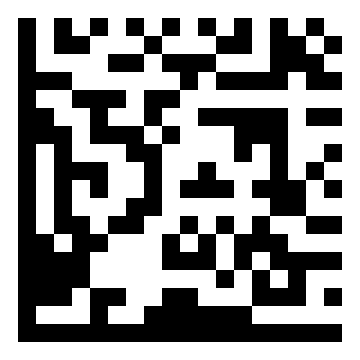
\includegraphics[width=0.90\linewidth]{abbildungen/tag18/gemischt_ascii.png}\\[4pt]
  {\small ASCII-Modus\\18×18, 17 Daten-CW}
\end{minipage}
\hspace{1.5cm}
\begin{minipage}[b]{0.28\linewidth}
  \centering
  
\includegraphics[width=0.75\linewidth]{abbildungen/tag18/gemischt_smart.png}\\[4pt]
  {\small Smart-Modus\\16×16, 12 Daten-CW}
\end{minipage}
\caption{„\texttt{BESTELLNR12345678}" — gleicher Inhalt, kleineres Symbol.
Der Smart-Encoder nutzt C40 für neun Buchstaben und Digit-Paar für acht
Ziffern.}
\end{figure}

Auch die reinen Vergleiche sind sehenswert:

\begin{figure}[h]
\centering
\begin{minipage}[b]{0.28\linewidth}
  \centering
  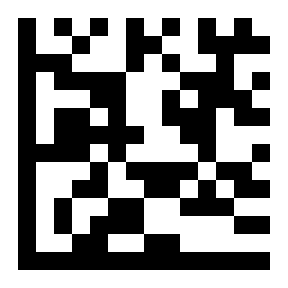
\includegraphics[width=0.90\linewidth]{abbildungen/tag18/ziffern_ascii.png}\\[4pt]
  {\small \texttt{"12345678"}\\ASCII: 14×14}
\end{minipage}
\hspace{1cm}
\begin{minipage}[b]{0.28\linewidth}
  \centering
  
\includegraphics[width=0.75\linewidth]{abbildungen/tag18/ziffern_smart.png}\\[4pt]
  {\small \texttt{"12345678"}\\Digit-Paar: 12×12}
\end{minipage}
\hspace{1cm}
\begin{minipage}[b]{0.28\linewidth}
  \centering
  
\includegraphics[width=0.65\linewidth]{abbildungen/tag18/text_smart.png}\\[4pt]
  {\small \texttt{"PRAKTIKUMSWOCHE"}\\C40: 16×16}
\end{minipage}
\caption{Links: dieselbe Ziffernfolge — vier statt acht Codewords.
Rechts: 15~Buchstaben im C40-Modus brauchen nur 12~Codewords statt~15
und passen damit in ein~16×16-Symbol statt~18×18.}
\end{figure}

% =============================================================
\section{Reflexion und Brücke zu Tag 19 \normalfont(\textit{≈ 10 min})}
% =============================================================

Du hast heute gelernt:

\begin{itemize}
\item Der \textbf{Digit-Paar-Modus} kodiert zwei Ziffern als ein
  Codeword (Werte 130–229). Das haliert den Platzbedarf reiner
  Ziffernfolgen.
\item Der \textbf{C40-Modus} kodiert drei Zeichen aus
  \{A–Z, 0–9, Leerzeichen\} als zwei Codewords. Er lohnt sich erst
  ab ca.\ sechs Zeichen im Segment, weil Latch und Unlatch je ein
  Codeword kosten.
\item \texttt{kodiere\_smart()} entscheidet pro Segment automatisch —
  Digit-Paar für Ziffernpaare, C40 für lange Buchstabenläufe,
  ASCII als sicherer Fallback.
\item Die \texttt{DatamatrixEncoderModi}-Klasse überschreibt nur
  eine einzige Zeile gegenüber dem Basis-Encoder. Den Rest — Padding,
  Reed-Solomon, Bitmap, PNG-Export — erbt sie unverändert.
\end{itemize}

\subsection*{Vorschau Tag 19}

Datamatrix ist nicht der einzige 2-D-Code der Welt. Der \textbf{QR-Code}
ist heute noch weiter verbreitet — auf Fahrkarten, Webseiten,
Restaurantmenüs. Beide nutzen Reed-Solomon, aber mit anderen Parametern
und einer ganz anderen Struktur:

\begin{itemize}
\item \textbf{Finder-Muster}: drei große Quadrate in den Ecken
  statt einer umlaufenden Rahmen-Linie
\item \textbf{Fehlerkorrektur-Level}: QR bietet vier Stufen (L, M, Q, H)
  statt eines festen ECC-Anteils
\item \textbf{Masking}: das Bitmuster wird nach festen Regeln
  invertiert, damit keine großen einfarbigen Flächen entstehen
\end{itemize}

Wir schauen, was beides gemeinsam hat und wo sie sich unterscheiden —
und warum Reed-Solomon in beiden steckt.
